\section{The algorithm}
In 1972 and 1974, the National Bureau of Standards (now the National Institute of Standards and Technology, or NIST) issued the first public request for an encryption standard. The result was DES \cite{NBS77}, arguably the most widely used and successful encryption algorithm in the world. However, due to advances in distributed key search techniques, the key was found to be too short for modern security applications.
Triple-DES emerged as a temporary solution in many high-security applications, such as banking, but it was too slow for some uses. More fundamentally, the 64-bit block length shared by DES and most other well-known ciphers opens it up to attacks when large amounts of data are encrypted under the same key.

Twenty years later, in 1997, NIST announced the Advanced Encryption Standard (AES) \cite{NIST97a}. NIST requested comments from the public on the proposed standard, and eventually issued a call for algorithms to satisfy the standard \cite{NIST97b}. NIST made all submissions public and eventually, through a process of public review and comment, chose a new encryption standard to replace DES. Twofish did not win, but made it as one of the five finalists in the 1997 competition.

Figure \ref{fig:twofish} shows the Twofish algorithm. It is a 16 byte / 128-bit block cipher with a variable key length between 128 and 256 bits. The cipher is a 16-round Feistel network also called a substitute-permute network. It has a bijective function F consisting of four key-dependent 8-by-8-bit S-boxes (Substitution-boxes) \cite{wiki_sbox}, a fixed 4-by-4 MDS (maximum distance separable) matrix over GF($2^8$) (Galois-field), a PHT (pseudo-Hadamard transform), bitwise rotations, and a carefully designed key schedule.

\begin{figure}[htp]
  \centering
  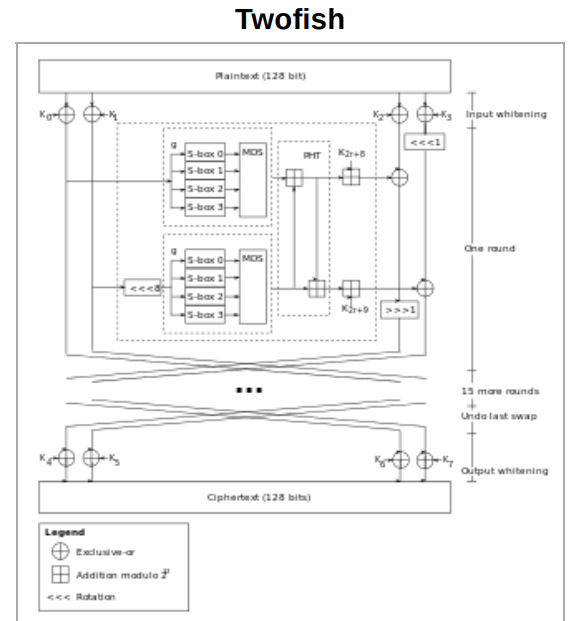
\includegraphics[scale=0.4]{Graphics/twofish.png}
  \caption{The Twofish algorithm}
  \label{fig:twofish}
\end{figure}
I will go over each of these building blocks, explaining what they are:

\subsection{Feistel Networks}
A Feistel network is a general method of transforming any function (usually called the F function) into a permutation. It was invented by Horst Feistel in 1973.

The fundamental building block of a Feistel network is the F function: a key-dependent mapping of an input string onto an output string. An F function is always non-linear and possibly non-surjective\footnote{A non-surjective F function is one in which not all outputs in the output space can occur.}:

\begin{equation*}
  F : \lbrace 0, 1\rbrace^{n/2} x \lbrace0, 1\rbrace^N -> \lbrace 0, 1\rbrace^{n/2}
\end{equation*}

where n is the block size of the Feistel Network, and F is a function taking n/2 bits of the block and N bits of a key as input, and producing an output of length n/2 bits. In each round, the “source block” is the input to F , and the output of F is XOR'ed with the “target block,” after which these two blocks swap places for the next round. The idea here is to take an F function, which may be a weak encryption algorithm when taken by itself, and repeatedly iterate it to create a strong encryption algorithm.  Two rounds of a Feistel network is called a \textbf{cycle}. In one cycle, every bit of the text block has been modified once.

\subsection{S-boxes}
An S-box is a table-driven non-linear substitution operation used in most block ciphers. S-boxes vary in both input size and output size, and can be created either randomly or algorithmically. S-boxes were first used in Lucifer by Horst Feistel, then DES, and afterwards in most encryption algorithms. Twofish uses four different, bijective, key-dependent, 8-by-8-bit S-boxes. These S-boxes are built using two fixed 8-by-8-bit permutations and key material.

\subsection{A small example}
Lets talk a little bit about the magic of substitute-permute networks. As the name implies, we first do a substitution followed by a permutation. I'll give a small example with a 2-by-2-bit S-box followed by a substitution.
Lets say you have a table of substitutions. 2 bits means we have 4 different values '00', '01', '10' and '11'.
So we do a mapping which could look like this:
\begin{table}[htp]
  \begin{center}
    \label{fig:small_subs_example}
    \begin{tabular}{|c|c|c|c|}
      \hline
      00 & 01 & 10 & 11 \\ \hline
      10 & 00 & 11 & 01 \\ \hline
    \end{tabular}
    \caption{2-by-2-bit S-box example.}
  \end{center}
\end{table}

This means that if we see '10' we substitute it to '11' and if we see '11' we substitute it to '01'. Thats the substitution part. \\
For the permutation part, lets say we have two of these 2-bit S-boxes. The output would be 2 bits from each, so we have 4 bits of output in total. The permutation is switching bits like this:
(* Insert permutation picture *)
%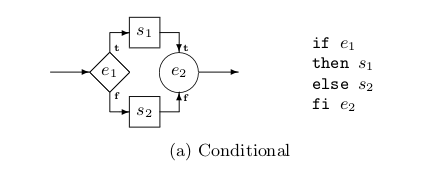
\includegraphics{permutation_example.png}[scale=0.7] \\
So if we want to substitute-permute the number 4 for example it would look like '0100', so the first Sbox would have input '01' and the second Sbox would have input '00'. This would result in the output of the first S-box being '00' and the output of the second S-box to be '10'. So the number 4 goes through the two S-boxes and comes out as a 2. Then it enters the permutation and becomes TODO: lorem ipsum

This constitutes one round of encryption. Now obviously this process is very easy to reverse if the substition table and the permutation table are public, so that is why we mix in keys. We XOR before the first encryption (input whitening), we XOR after each round and we XOR again after the last round (output whitening). Once you take the key away you can no longer reverse the process.

Twofish uses 16 rounds and AES uses 10-14 rounds. The tradeoff here is obviously speed. If you use too few rounds the encryption will be easier to break, but if you use too many it will be slow.


\subsection{MDS Matrices}
An MDS matrix is a linear mapping from a field elements to b field elements. It produces a composite vector of a + b elements with the property that for each non-zero vector there will be atleast b + 1 non-zero elements.
What this means is that the "distance" between two distinct vectors produced by the MDS mapping is atleast b + 1.
It is provable that no mapping can have a larger minimum distance between two distinct vectors and that is why we call it maximum distance seperable.
Twofish uses a 4-by-4 MDS matrix over GF ($2^8$) called the Reed-Solomon (RS) error-correcting codes.

\subsection{Pseudo-Hadamard transforms}
The 32-bit pseudo-Hadamard transform (PHT) that Twofish uses is a mixing operation that given two inputs a and b updates the two values as follows:
%\begin{equation*}
%  a' = a + b mod 2^{32} \\
%  b' = a + 2b mod 2^{32}
%\end{equation*}

\subsection{Whitening}
Input/output whitening is done by XOR'ing 128 bits of subkey, which is not used in any of the rounds, with part of the expanded key before the first round and after the last round. It was shown in 1996 by Rivest \cite{KR96} that whitening made it substantially harder for attackers to do keysearch attacks.

\subsection{Key schedule}
The key schedule is the means by which the key bits are turned into round keys that the cipher can use.  Twofish needs a lot of key material, and has a complicated key schedule. To facilitate analysis, the key schedule uses the same primitives as the round function.

There are two types of keys used for the twofish algorithm. It uses a user-supplied global key M of 128 bits to generate two sets of subkeys S and K. S has two subkeys $S_0$ and $S_1$ which are fixed during the entire encryption and decryption process. $S_0$ and $S_1$ are used in the S-boxes inside the g function. The key schedule performs a key expansion to make K, which is a 40-word expanded key where each word consists of 32 bits. I'll refer to these as $K_0$ through $K_{40}$. Words 0-7 are used for input / output whitening whilst the remaining 32 words are passed on to the bijective function F two at a time during the 16 rounds of encryption. \\

The generation of S is done by multiplication in the Galois field GF $(2^8)$ where the primitive polynomial is $x^8 + x^6 + x^3 + x^2 + 1$.

TODO: I have not implemented key schedule as there is a problem with galois field multiplication when b == 0 which happens in the key schedule.
%\begin{lstlisting}
% This is what we want if we use key schedule
%     __       _____
%0 - |ks| --  |ks^-1| - 0
%k - |__| --  |____ | - k
%          |
%          |
%   d  ---enc ---- c
%\end{lstlisting}
